\section{Test-beam Setup and Experimental Apparatus }
\label{sec:tbeam}

We performed the measurements at the H2 beamline of the CERN North-Area testbeam facility
and the T9 beamline of the CERN East-Area testbeam facility. They provide secondary electron beams 
from the Proton Synchrotron (PS) and Super Proton Synchrotron (SPS)
of energies ranging from $2$~GeV to $200$~GeV. The secondary beams are composed of 
a mixture of electrons, pions, and muons. 

Trigger counters made of photomultipliers coupled to $4 \mathrm{cm}\times 4 \mathrm{cm}$ 
plastic scintillators are used 
to initiate the read out of the data acquisition (DAQ) system. The DAQ system
uses a CAEN V1742 switched capactor digitizer based on the DRS4 chip~\cite{DRS}. Wire chambers
are used to measure the position of each incident beam particle in the plane transverse
to the beamline. A stack of lead or tungsten absorbers of different thicknesses are 
placed about $5$~mm in front of the CdTe sensor, which is 
enclosed within an aluminum box covered by copper foil. We amplified the size of the
signals from the CdTe sensor using a Hamamatsu C5594 amplifier~\cite{HamaAmpDataSheet} with a bandwidth of
$1.5$~GHz and providing a voltage gain of $36$~dB. A micro-channel plate photomultiplier (MCP-PMT)
detector is used to provide a very precise reference timestamp. At the T9 beamline,
a Hamamatsu R3809U MCP-PMT~\cite{HamaMCPDataSheet} is placed just upstream of the absorber material. 
At the H2 beamline a Photek 240 MCP-PMT~\cite{PhotekDataSheet} is used, which contains a significant 
amount of absorber material (about 1.8 radiation lengths), and is therefore placed 
just downstream of the CdTe sensor to avoid inducing an early electromagnetic shower.
The precision of the time measurement for both types of MCP-PMT's is less than 
$10$~ps~\cite{MCPShowerMaxPaper}. The purity of the electron beam at the T9 beamline is
significantly lower than at the H2 beamline, and therefore we use a LYSO crystal
optically coupled to an MCP-PMT as a means of discriminating the electrons from the pions
in the beam. The schematic diagrams of the experimental setups at H2 and T9 
are shown in Figure~\ref{fig:BeamSchematicDiagram}. 


%Fig: Diagram of detector elements
\begin{figure}[htbp] 
\centering
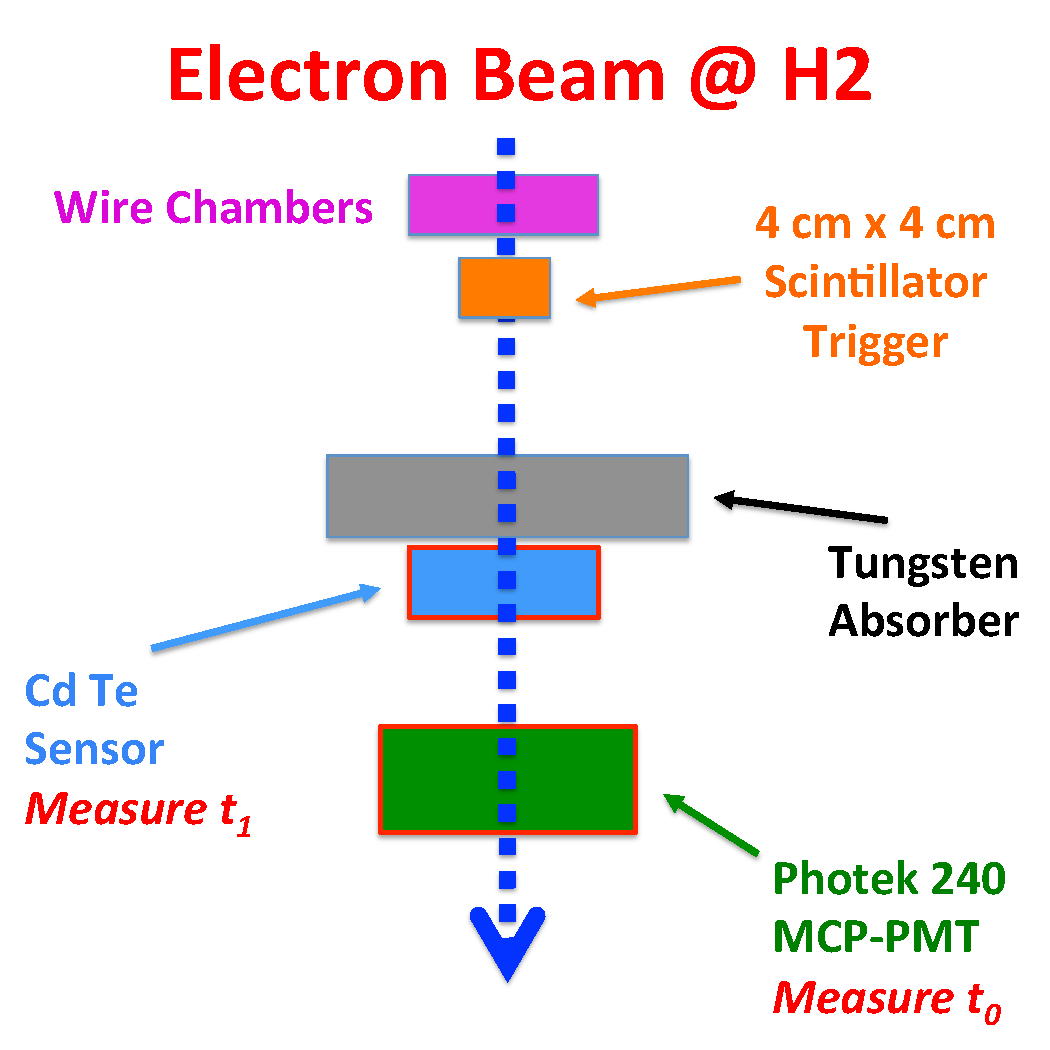
\includegraphics[width=0.49\textwidth]{figures/H2_BeamSchematicDiagram.pdf} 
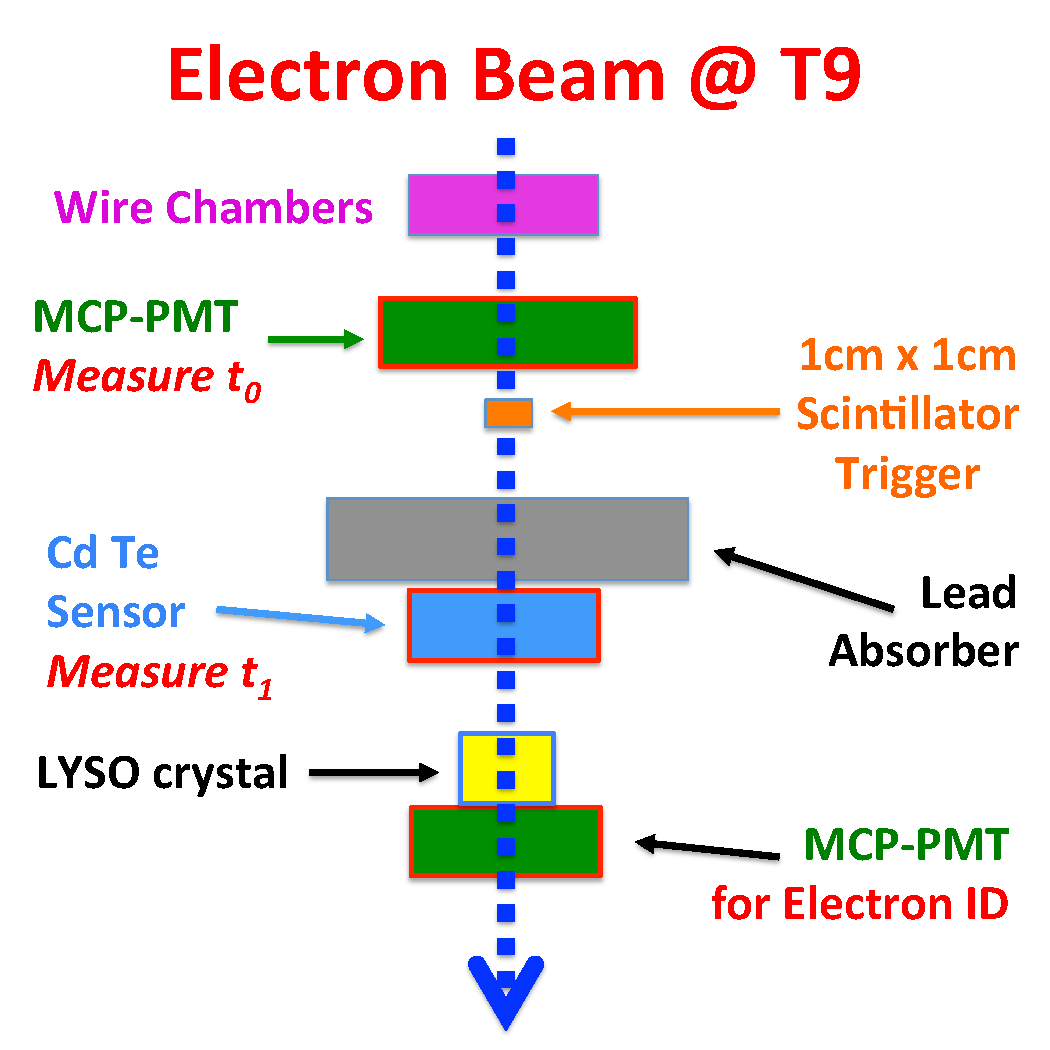
\includegraphics[width=0.49\textwidth]{figures/T9_BeamSchematicDiagram.pdf} 
\caption{Schematic diagrams of the test-beam setups at H2 (left) and T9 (right) are shown. 
The timestamps $t_0$ and $t_1$ are defined in Section~\ref{sec:reco}.} 
\label{fig:BeamSchematicDiagram} 
\end{figure} 


The X and Y position measurements from the wire chamber are used to determine the location
of the CdTe sensor relative to the beam and to align the beam. In 
Figure~\ref{fig:BeamSensorPosition}, we show the average amplitude measured in the
CdTe sensor as a function of the X and Y positions as measured by the wire chamber. Based
on these plots, we can restrict our measurements to those electrons whose impact point is close
to the center of the CdTe sensor.

%Fig: Beam profile X-Y plot
\begin{figure}[htbp] 
\centering
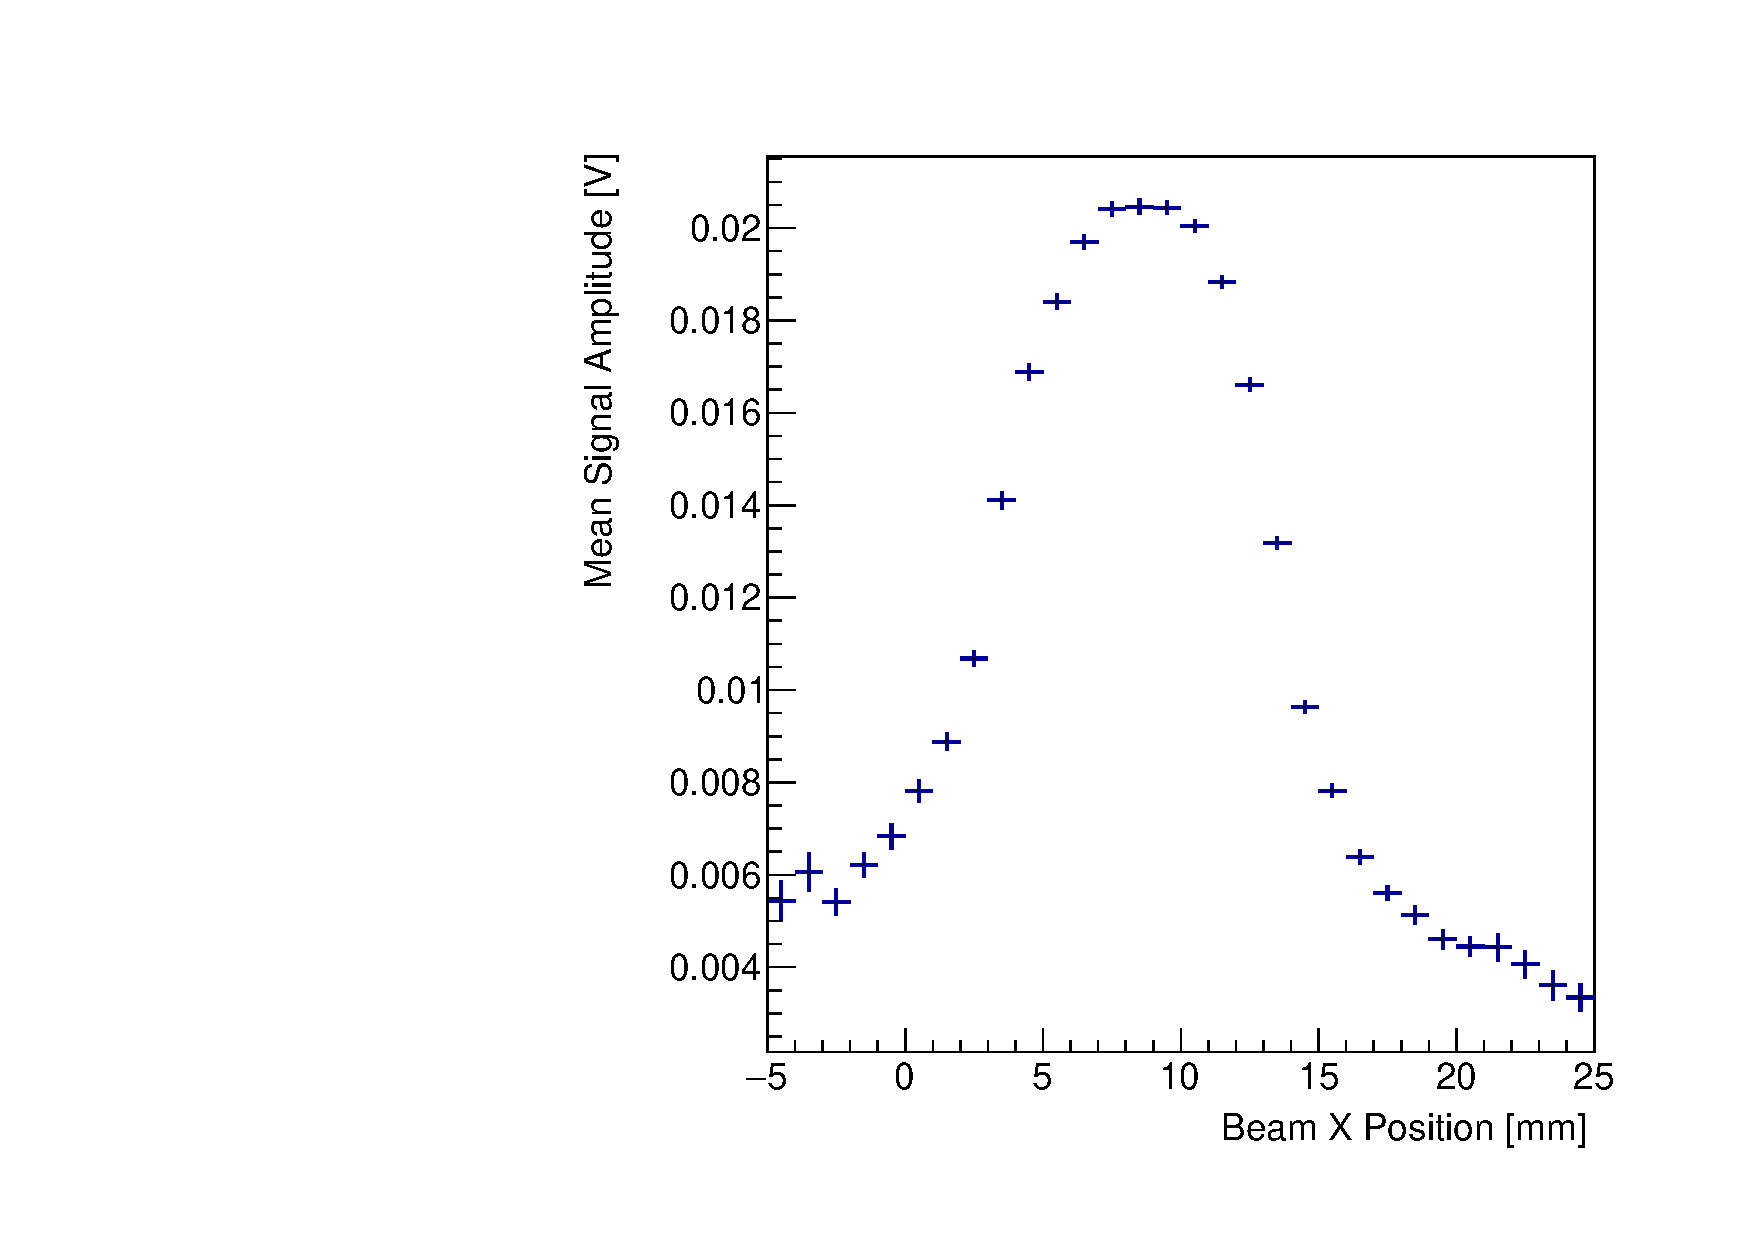
\includegraphics[width=0.49\textwidth]{figures/SensorXProfile.pdf} 
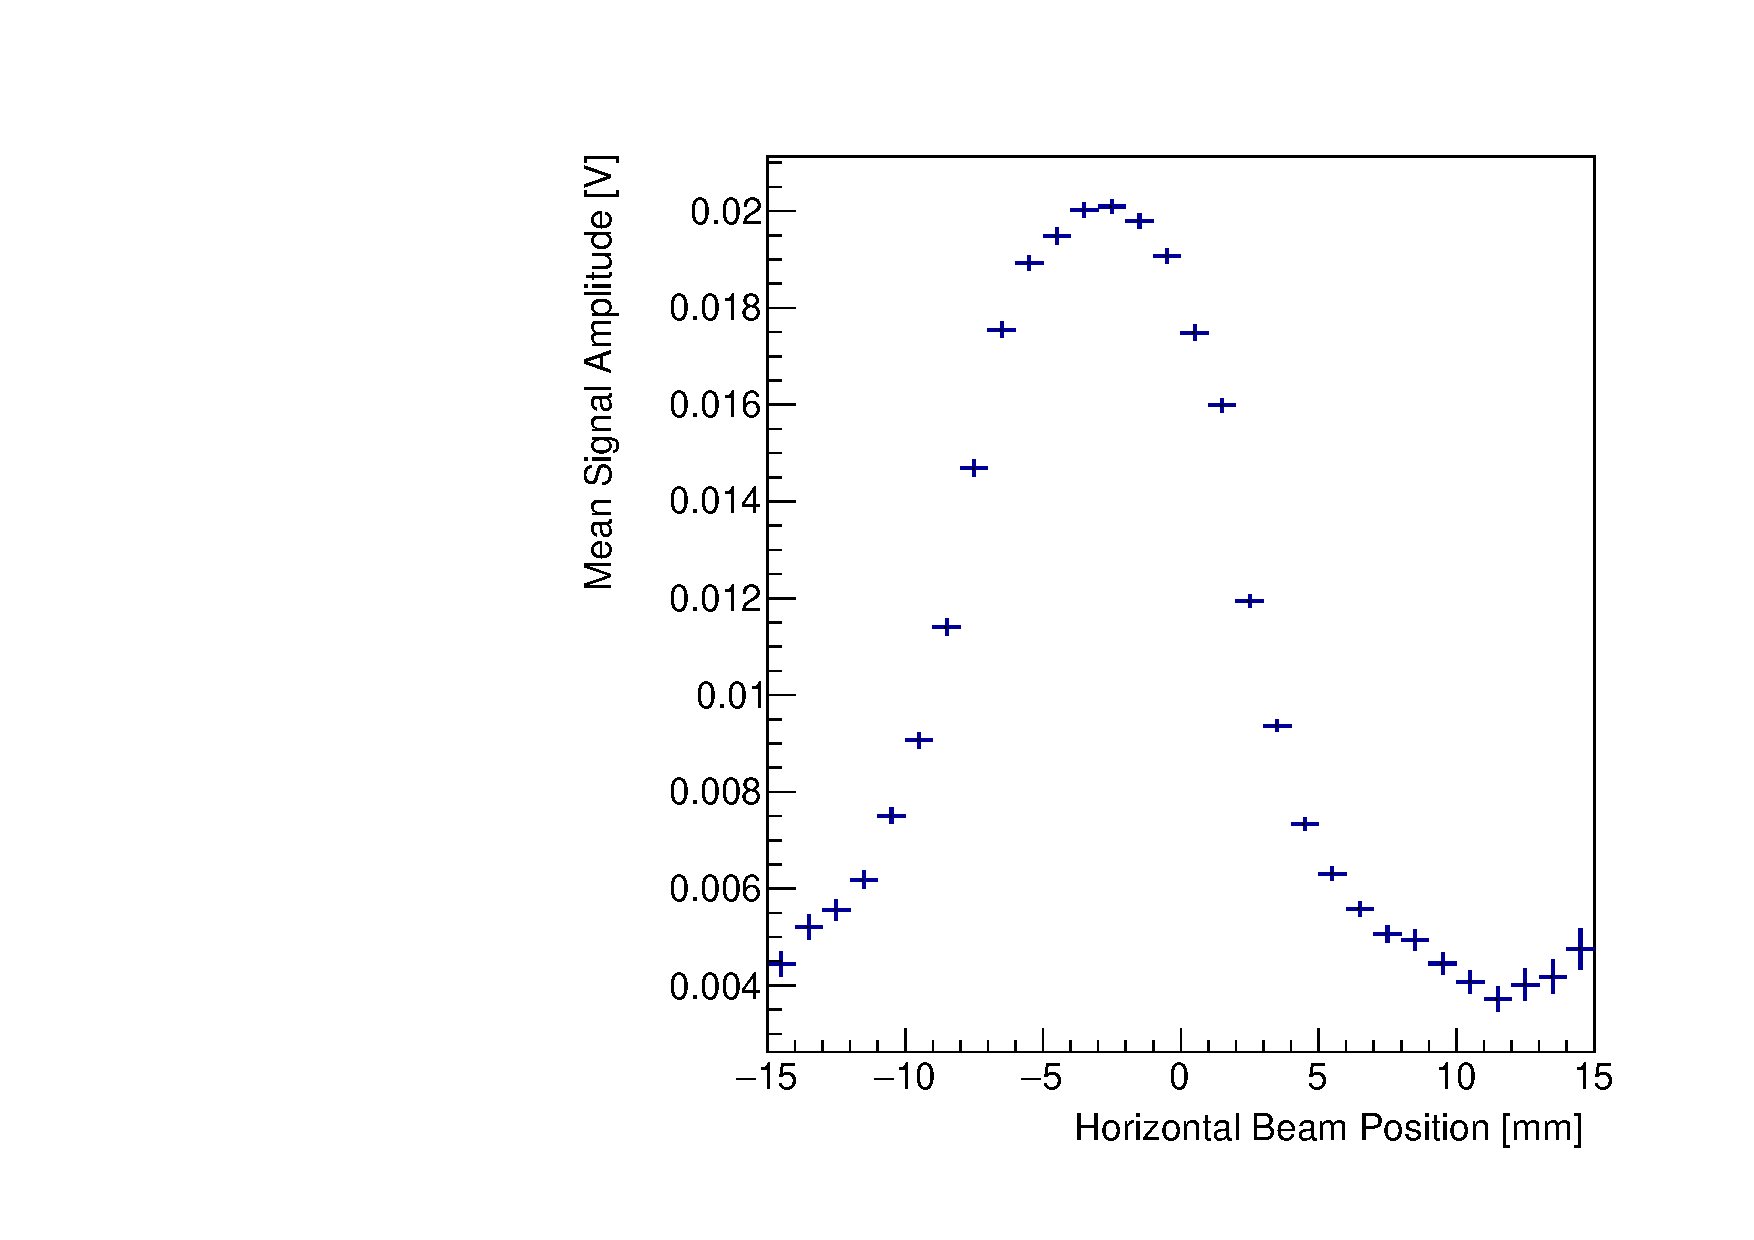
\includegraphics[width=0.49\textwidth]{figures/SensorYProfile.pdf} 
\caption{The average amplitude measured in the CdTe sensor is plotted as a function of 
the horizontal and vertical positions of the beam particle as measured by the wire chamber.} 
\label{fig:BeamSensorPosition} 
\end{figure} 

